\chapter{The AMBER Experiment}\label{chap:chapter 2}
\acresetall

\section{Overview of the AMBER Experiment}

The AMBER (Apparatus for Meson and Baryon Experimental Research) experiment, designated NA66, is a fixed-target experiment at CERN. It is located at the Super Proton Synchrotron (SPS) in the North Area of CERN, shown in \ref{fig:LHC}. It was approved in 2020 as a multi-purpose facility dedicated to precision studies in hadron physics. Building upon the spectrometer and infrastructure of the former COMPASS experiment, AMBER combines existing detector systems with substantial upgrades to address a broad physics program. It can be operated with both muon and hadron beams. These come from the M2 beam line, which is directly connected to the SPS.

\begin{figure}[h]
    \centering
    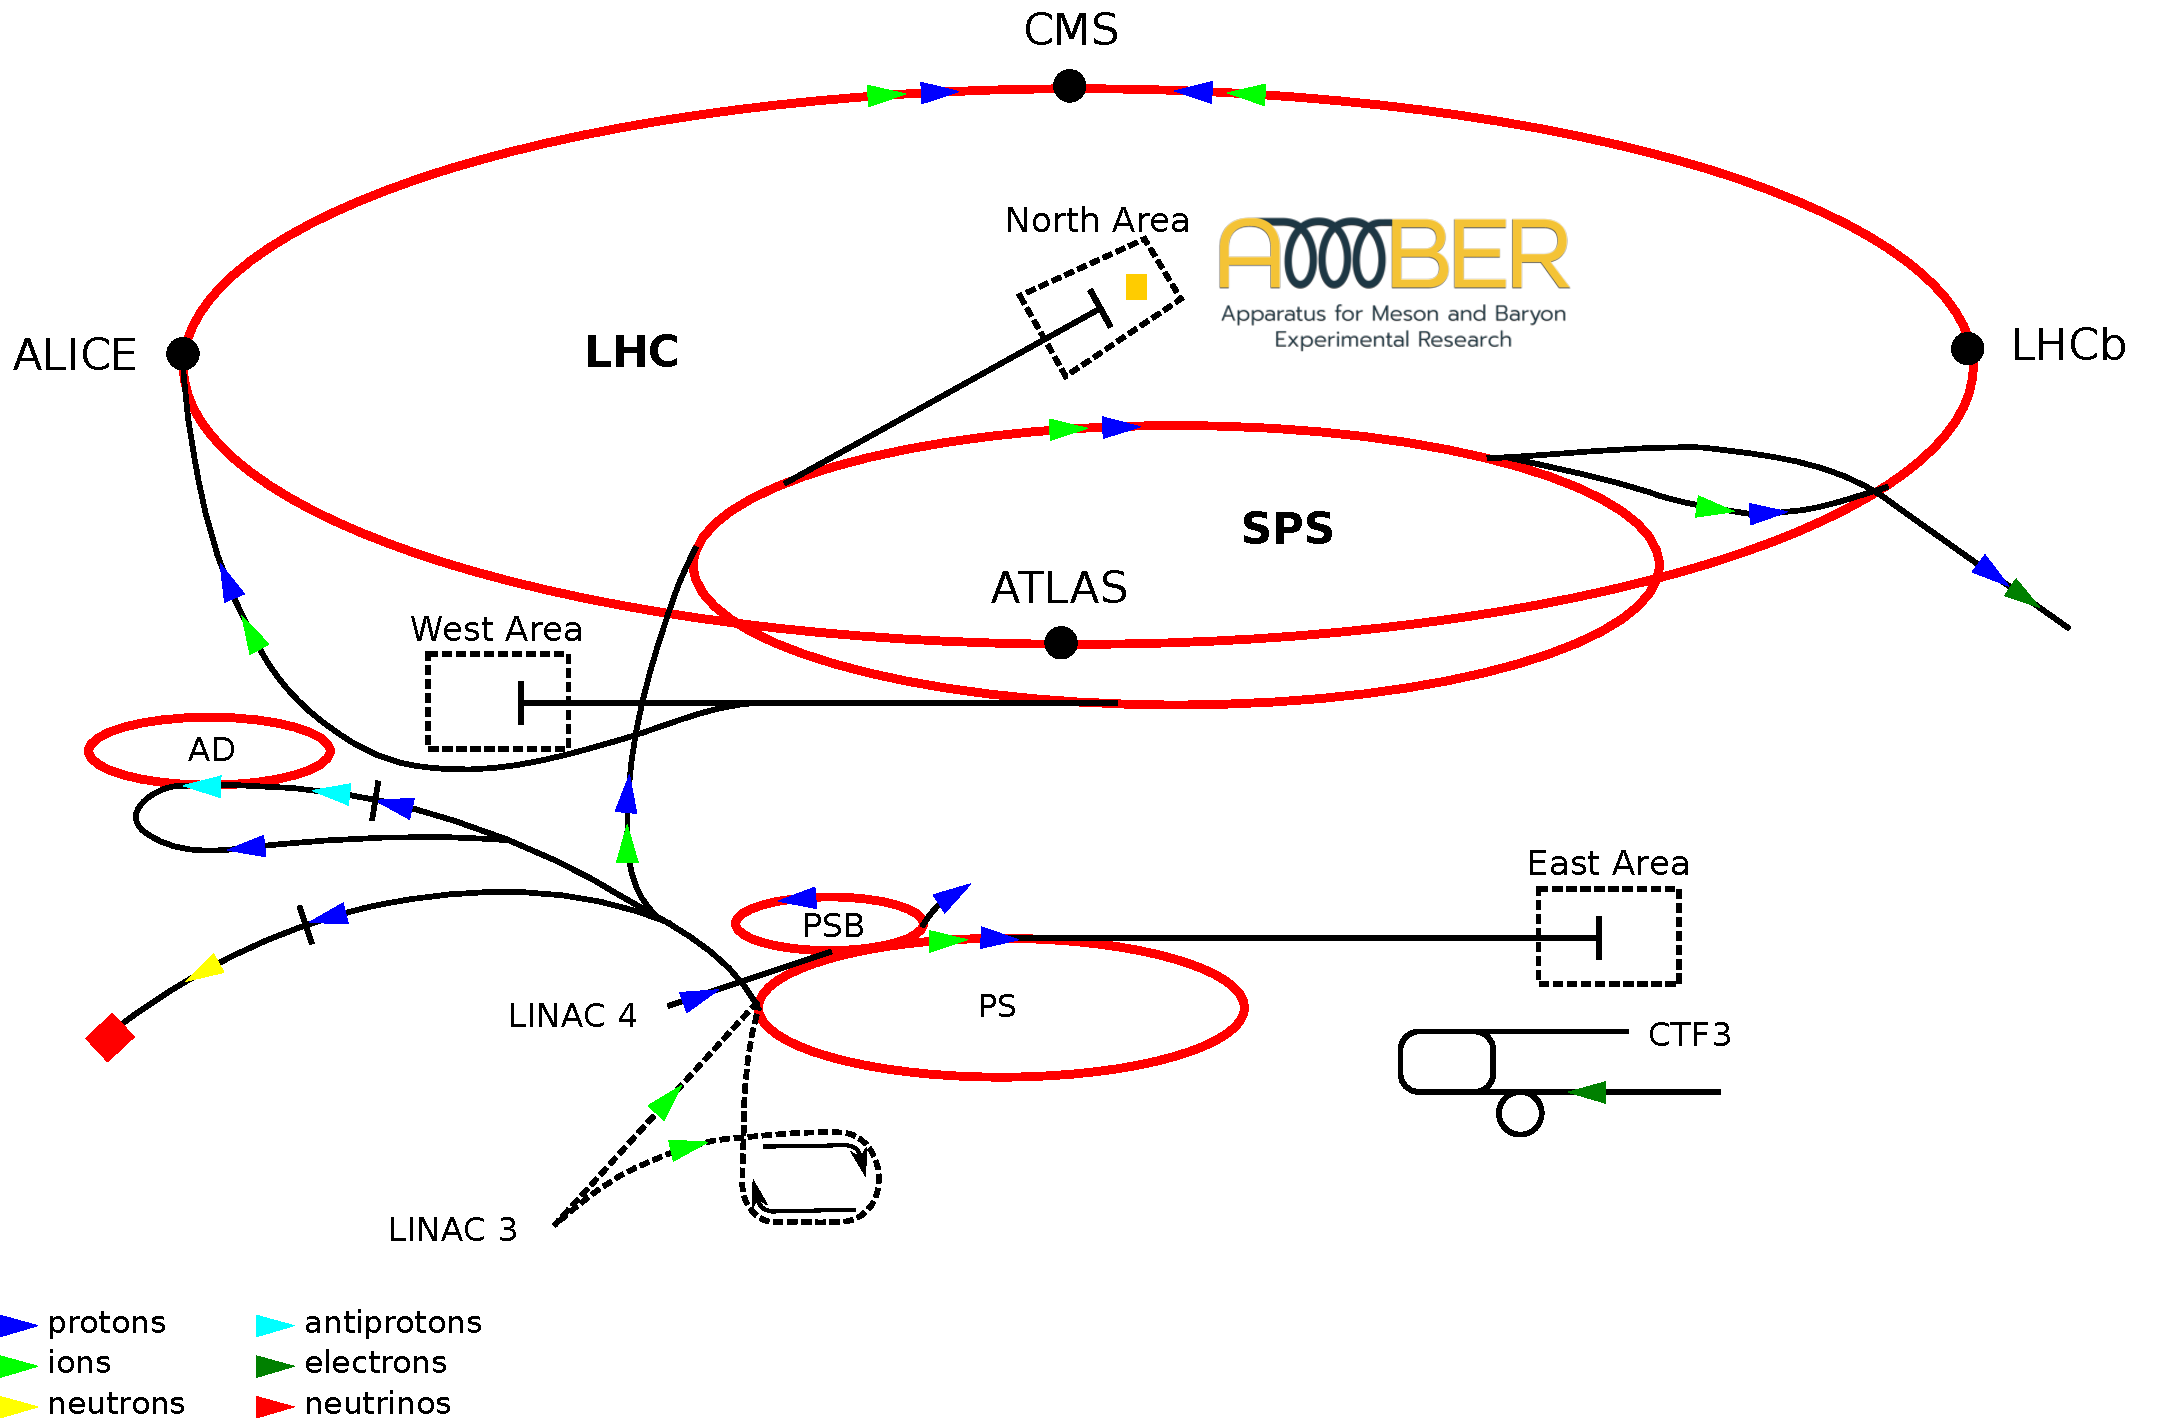
\includegraphics[width=0.8\textwidth]{figures/Cern-accelerator-complex.pdf}
    \caption{Location of the AMBER experiment within the CERN accelerator complex. Figure adapted from \cite{LHC}.}
    \label{fig:LHC}
\end{figure}

In Phase-1 (2022-2026), the experiment focuses on measurements of antiproton production cross sections, investigations of the partonic structure of mesons through Drell-Yan processes, hadron spectroscopy, and a high-precision \ac{PRM}. AMBER aims to determine the proton charge radius using elastic muon-proton scattering. The measurement covers a very low four-momentum-transfer region, where the electric form factor is particularly sensitive to the proton's charge radius.

After Long Shutdown 3, in Phase-2, AMBER plans to extend its physics program towards measurements requiring high-intensity hadron beams. The main objectives include precision studies of the internal structure of hadrons, such as the three-dimensional partonic structure of mesons and baryons, as well as further investigations of hadron production mechanisms.

\section{Experimental Setup for the Proton Radius Measurement}
The proton-radius measurement is performed using a \SI{100}{GeV} muon beam. The beam is delivered to the detector in spills. A spill refers to a single period during which the beam is extracted from the accelerator and delivered to the experiment. For AMBER, a spill is approximately \(\qty{4.8}{\second}\) long. Therefore, an intensity of approximately \(4\times10^6\) muons per spill corresponds to an average rate of about \(8.3\times10^5\) muons per second that hit the target during the spill. The beam is provided by the M2 beam line and is directed onto an active hydrogen target operated at a pressure of \SI{20}{bar}. The high pressure increases the density of hydrogen atoms in the target, thereby increasing the probability of elastic muon-proton scattering. Since hydrogen provides a clean proton target, it allows the proton kinematics to be reconstructed without additional nuclear effects. The scattered muon is measured with the COMPASS spectrometer, while the recoil proton is reconstructed inside the target using a \ac{TPC}. An overview of the experimental setup is shown in \autoref{fig:setup}.

The direction of the incoming beam defines the longitudinal axis of the experiment. Detector components located before the interaction point with respect to the beam direction are referred to as upstream, whereas components located after the interaction point are called downstream.

The main detector components relevant for the \ac{PRM} are described in the following.

\begin{figure}[h]
    \centering
    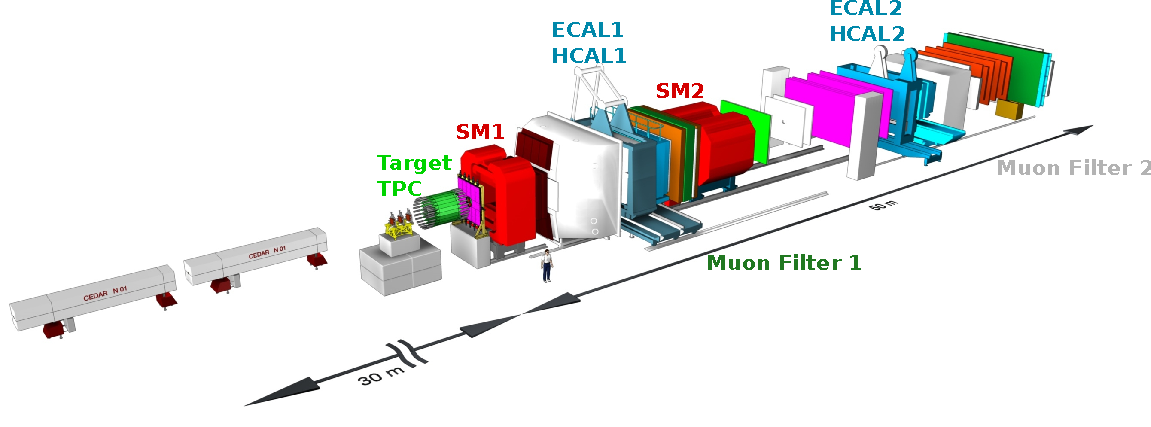
\includegraphics[width=1.\textwidth]{figures/setup.pdf}
    \caption{LALALA. Figure adapted from \cite{setup}.}
    \label{fig:setup}
\end{figure}

\paragraph{Combined Tracking Stations}

Four combined tracking stations surround the target region, with two stations located upstream and two downstream of the \ac{TPC}. Their primary purpose is to reconstruct the trajectories of the incoming and scattered muons with high spatial and temporal precision.

Each tracking station combines a silicon pixel detector with several layers of scintillating fibers. The pixel detector provides excellent spatial resolution for determining the interaction vertex and scattering angles. The scintillating fibers, consisting of thin plastic fiber ribbons connected to photomultipliers, offer a time resolution of less than \SI{1}{ns}. This precise timing is crucial to disentangle individual beam particles and match track segments with the \ac{TPC} signals, where the total electron drift time is on the order of \SI{100}{\micro\second}.

\paragraph{Time Projection Chamber}

The \ac{TPC} serves as an active hydrogen target. It is \qty{2.3}{\meter} long and operated with hydrogen gas at a pressure of \qty{20}{\bar}. The chamber consists of four cylindrical drift cells, each with a length of \qty{40}{\centi\meter} and a diameter of \qty{60}{\centi\meter}.

When a charged particle traverses the hydrogen gas, it ionizes the gas molecules and creates electron-ion pairs along its trajectory. An electric drift field causes the liberated electrons to move towards the readout plane, where their arrival time and position are measured. From these signals, the three-dimensional trajectory of the recoil proton can be reconstructed.

Since the proton loses energy as it traverses the gas, its kinetic energy can be determined from the measured ionization. Together with the reconstructed momentum, this allows the proton kinematics and the squared four-momentum transfer \(Q^2\) to be determined with high precision.

\paragraph{Spectrometer Magnets}

Downstream of the target, the spectrometer consists of two dipole magnets, SM1 and SM2. During the \ac{PRM}, the first magnet (SM1) is switched off to prevent small-angle scattered muons from being deflected before reaching the downstream target tracking stations. Consequently, momentum reconstruction for the scattered muon is performed exclusively using the second dipole magnet, SM2, and the measurements of the tracking detectors.

This single-magnet deflection scheme is well-suited for elastic muon-proton scattering at low \(Q^2\), as the process is strongly forward-peaked, giving rise to small scattering angles and high forward momenta.

\paragraph{Electromagnetic and Hadronic Calorimeters}

The spectrometer features a two-stage calorimeter system containing two electromagnetic calorimeters (ECAL1 and ECAL2) and two hadronic calorimeters (HCAL1 and HCAL2). Calorimeters measure the energy of particles through the detection of the energy deposited in active detector material.

Electromagnetic calorimeters are designed to absorb and measure the energy of light particles, primarily electrons, positrons, and photons. High-energy electrons lose energy via Bremsstrahlung, while photons convert into electron-positron pairs. This alternating process initiates an electromagnetic shower characterized by the material's radiation length. The total deposited energy is related to the incident particle energy and can be used to reconstruct photons and electrons.

The AMBER setup employs lead-glass blocks and sampling Shashlik-type modules (alternating layers of lead absorber and plastic scintillator). The light generated by Čerenkov radiation or scintillation inside the absorber material is collected by photodetectors (such as photomultipliers or avalanche photodiodes) and converted into an electrical signal proportional to the particle's energy.

In the context of the \ac{PRM}, the electromagnetic calorimeters are particularly important because photons emitted during radiative muon-proton scattering have to be detected and studied. These photons modify the experimentally reconstructed kinematics and therefore play an important role in the determination of radiative corrections. In particular, ECAL2 provides information on photons emitted at larger distances downstream of the target and is an essential detector for the studies presented in this thesis.

Hadronic calorimeters measure the energy of strongly interacting particles (hadron species such as protons, pions, and kaons). Hadrons interact with atomic nuclei inside dense absorber materials (iron or lead), generating a hadronic cascade. Although they are not the primary detectors for the proton-radius measurement, they contribute to particle identification and background suppression within the spectrometer.

\paragraph{Muon Filters}

To ensure unambiguous identification of scattered muons, the spectrometer incorporates two dedicated muon filter systems: MF1 (upstream) and MF2 (downstream).

Each muon filter consists of a thick iron or concrete absorber wall followed by tracking detectors. Strongly interacting hadrons and remaining electromagnetic shower components undergo nuclear interactions or showers and are completely absorbed within the material. In contrast, high-energy muons behave as minimum ionizing particles, penetrating the absorber material with minimal energy loss. 

By matching tracks recorded in the tracking detectors directly behind the absorber walls with momentum tracks reconstructed via SM2, MF1 and MF2 provide a clean and highly efficient identification of the scattered muon.